%%%%%%%%%%%%%%%%%%%%%%%%%%%%%%%%%%%%%%%%%%%%%%%%%%%%%%%%%%%%%%%%%%
\section{TensorFlow Lite Delegate Implementation and Operation}

TensorFlow, as an open-source framework, provides extensible interfaces to optimize the execution of specific parts of a model on various hardware types. Within this structure, delegates are critical components that help TensorFlow Lite to efficiently reroute specific tensor operations to be run on specialized hardware accelerators, rather than the default \gls{cpu}.

This appendix dives into the implementation and operation of the TensorFlow Lite delegate interface for the proposed \gls{tp}.

\subsection{Implementation}

In the TensorFlow ecosystem, a delegate serves as a bridge connecting hardware and software, illustrated in \Fig{fig:sw_stack_appendix}. In this framework, specific tensor operations are offloaded to specialized hardware like \glspl{gpu}, \glspl{npu}, and custom accelerators such as the \gls{tp}. To harness the full potential of the proposed \gls{tp}, it is imperative to provide a tailored TensorFlow Lite delegate.

\begin{figure}[h!]
	\centering
	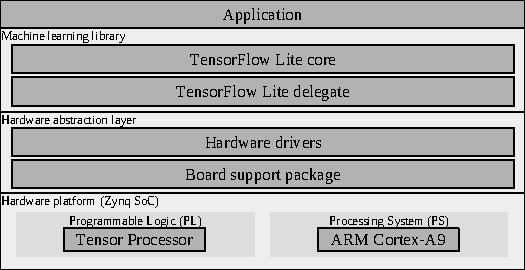
\includegraphics[width=0.5\textwidth]{./chapters/cnn_accelerator/figures/sw_stack.pdf}
	\caption{High level embedded software architecture.}
	\label{fig:sw_stack_appendix}
\end{figure}

The delegate interface identifies operations eligible for offloading and redirects them to the specialized hardware, as depicted in \Fig{fig:sw_stack_flowchart_apendix}.

\begin{figure}[h!]
	\centering
	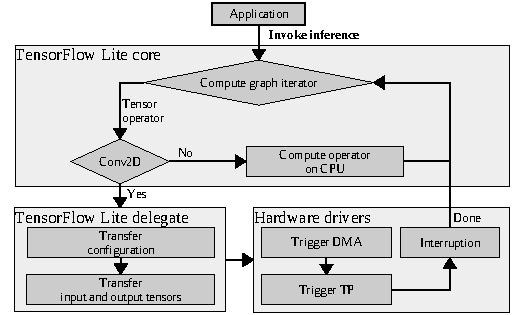
\includegraphics[width=0.5\textwidth]{./chapters/cnn_accelerator/figures/sw_stack_flowchart.pdf}
	\caption{Software flowchart.}
	\label{fig:sw_stack_flowchart_apendix}
\end{figure}


\subsection{Initialization}

As depicted in \Fig{fig:sw_tf_delegate_initialize}, the process commences by enabling the delegate interface at the application layer. Subsequently, the MicroInterpreter module creates and initializes the \gls{tp} delegate instance. During this phase, the \gls{tp} and \gls{dma} hardware drivers are also instantiated and set up.

\begin{figure}[h!]
	\centering
	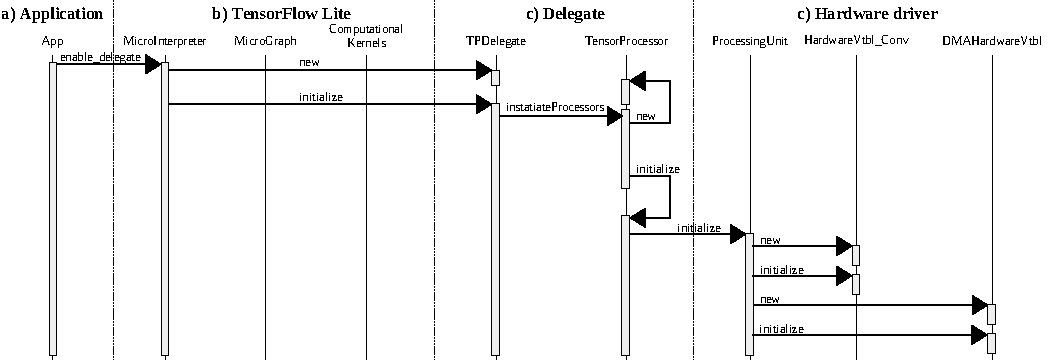
\includegraphics[width=\textwidth]{./figures/sequence_initialize_tf_delagate.pdf}
	\caption{Sequence diagram of TensorFlow delegate initialization.}
	\label{fig:sw_tf_delegate_initialize}
\end{figure}

\subsection{Operation}

During operation, TensorFlow executes the computational graph or model graph. The graph is a \gls{ml} model presentation, where nodes represent operations and edges symbolize the tensors that flow between these operations. Essentially, this graph provides a visual representation of how data is processed and transformed as it moves through the various operations of a \gls{ml} model.

The execution of the compute graph is depicted in \Fig{fig:sw_tf_delegate_execution}. Driven by the application layer, the MicroInterpreter module invokes the subgraph execution. The procedure involves:

\begin{enumerate}
	\item Traversing through each node in the compute graph.
	\item Assessing the tensor operator of each node and delegating the computation of \textit{Conv2D} operations to the \gls{tp}.
\end{enumerate}

\begin{figure}[h!]
	\centering
	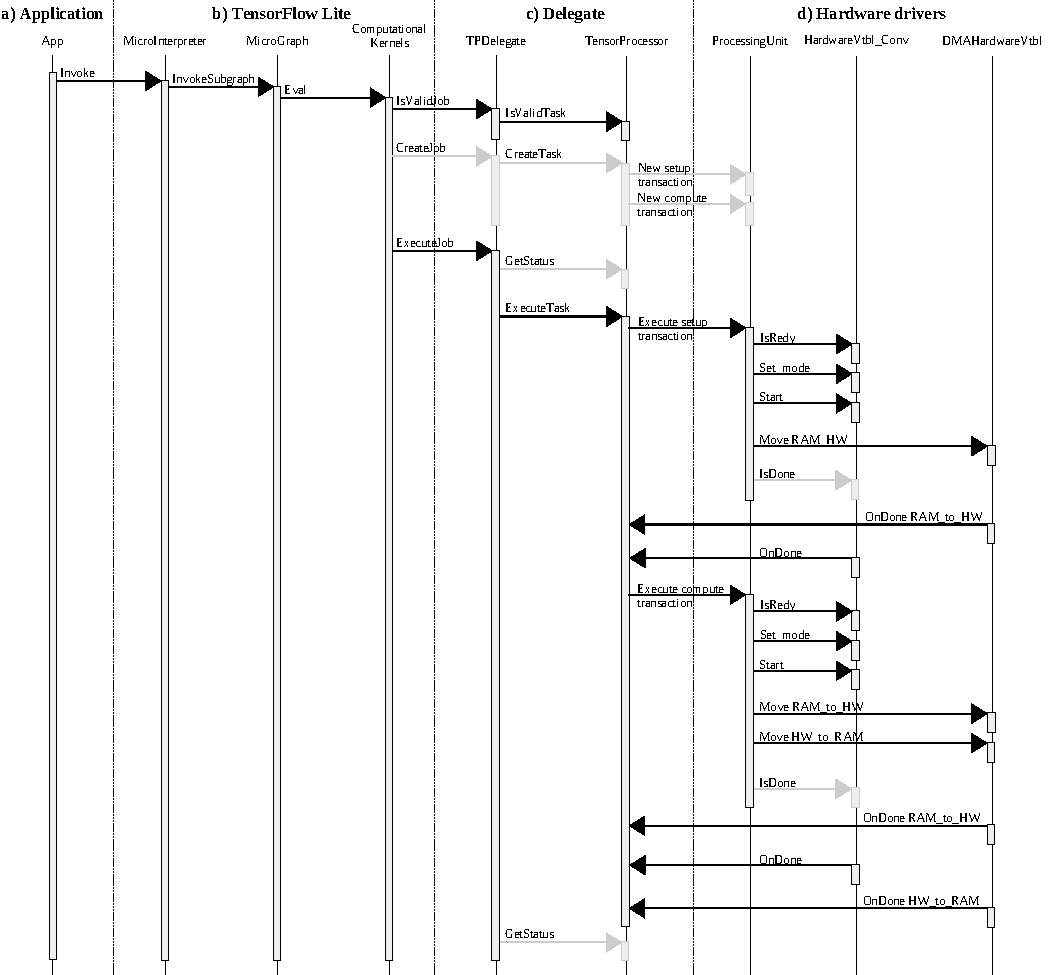
\includegraphics[width=\textwidth]{./figures/sequence_tfl_delegate_acceleration.pdf}
	\caption{Sequence diagram of TensorFlow delegate execution.}
	\label{fig:sw_tf_delegate_execution}
\end{figure}

When the delegate operates the \gls{tp}, it creates a 'Job' object. This object, serving as a container, consists of multiple tasks tailored for the \gls{tp}. Each task contains two data movement transactions that orchestrates:

\begin{itemize}
	\item \textbf{Setup Transaction:} Here, the \gls{dma} transfers the setup buffer (as illustrated in \Fig{fig:setup_transaction}) from the \gls{ram} to the \gls{tp} to establish a groundwork for the upcoming computations. See \Fig{fig:sw_tp_delegate_job} (a).
	\item \textbf{Compute Transaction:} As the core of the operation, the input tensor gets streamed to the \gls{tp} via the \gls{dma} TX channel. Concurrently, the output tensor flows out from the \gls{tp}, to the \gls{dram} through the \gls{dma} RX channel. See \Fig{fig:sw_tp_delegate_job} (b).
\end{itemize}

\begin{figure}[h!]
	\centering
	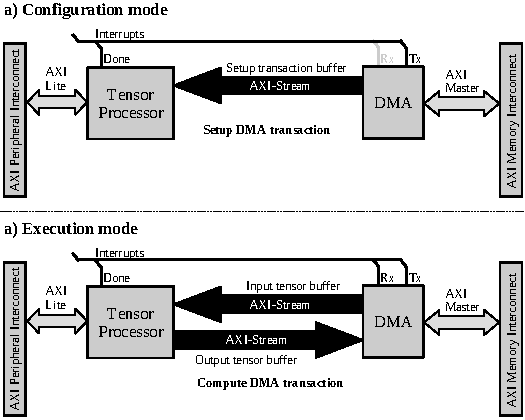
\includegraphics[width=0.5\textwidth]{./figures/task_execution.pdf}
	\caption{Tensor Processor task execution. (a) Setup transaction. (b) Compute transaction.}
	\label{fig:sw_tp_delegate_job}
\end{figure}

\begin{figure}[h!]
	\centering
	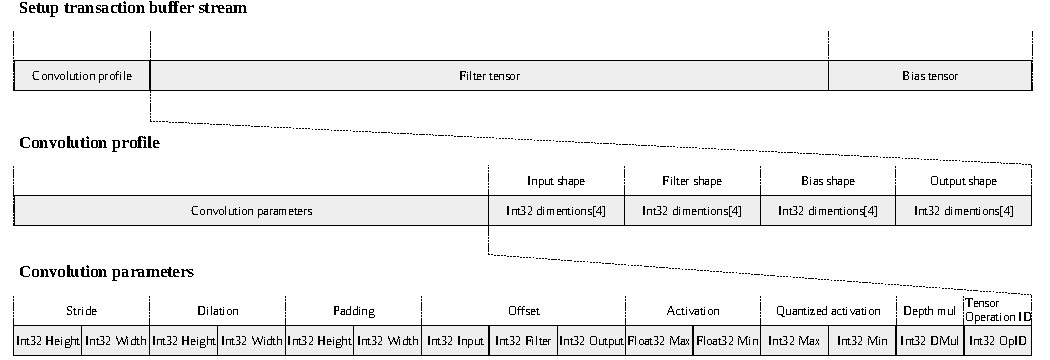
\includegraphics[width=\textwidth]{./figures/setup_transaction_buffer_stream.pdf}
	\caption{Setup transaction buffer stream.}
	\label{fig:setup_transaction}
\end{figure}

\subsection{Software Classes}
The collaboration diagram in \Fig{fig:sw_tp_delegate} offers a visual representation of the relationships between the delegate class implemented for the \gls{tp}. This diagram instrumental in understanding the interactions between classes and can be insightful for developers and researchers who aim to customize or extend the TensorFlow Lite delegate for specialized use-cases.

In this diagram, the central class is the `TPDelegate`, representing the delegate designed for the proposed custom \gls{tp}. This delegate interacts with a variety of other classes, facilitating tensor operations, memory management, and hardware tasks.

\begin{figure}[h!]
	\centering
	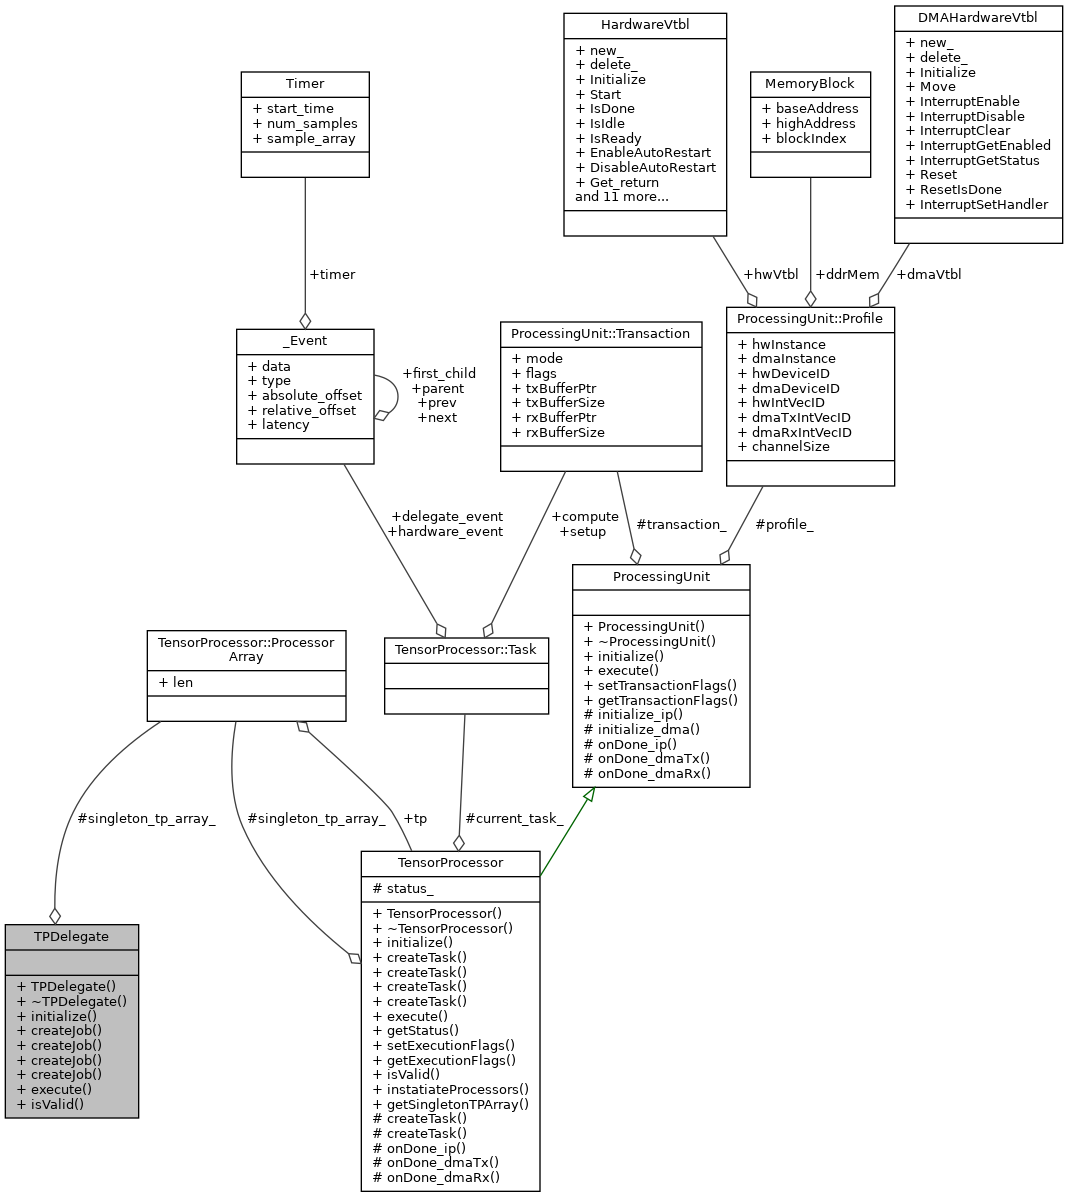
\includegraphics[width=\textwidth]{./figures/class_t_p_delegate__coll__graph.png}
	\caption{Collaboration diagram of TensorFlow delegate classes.}
	\label{fig:sw_tp_delegate}
\end{figure}


In conclusion, the TensorFlow Lite delegate for \gls{tp} encapsulates the mechanisms of software-hardware synergy, pushing the efficient neural network execution on custom hardware platforms.
%%%%%%%%%%%%%%%%%%%%

%%%%%%%%%%%%%%%%%%%%%%%%%%%%%%%%%%%%%%%%%%%%%%%%%%%%%%%%%%%%%%%%
\section{SbS algorithm}
\label{chap:appendix}
The SbS network inference is described in \Algo{alg:inference}, while spike production and layer update are described in \Algo{alg:spike} and \Algo{alg:update}, respectably.

\begin{algorithm}[t]
	\caption{SbS network inference.} \label{alg:inference}
	
	\begin{algorithmic}
		\SetAlgoLined
		\renewcommand{\algorithmicrequire}{\textbf{input:}}
		\renewcommand{\algorithmicensure}{\textbf{output:}}
		\REQUIRE Layers of the network as $H^l$, where\\
		$l$ is the layer index.
		\REQUIRE $N_{L}$ as the number of layers.
		\REQUIRE $N^l_{X}, N^l_{Y}$ as the size of layers.
		\REQUIRE $N_{Spk}$ as the number of spikes for inference (iterations).
		\ENSURE $H^l$.
		\FOR {$t = 0$ \textbf{to} $N_{Spk}-1$}
		\STATE \textit{Initialization of $H^l(i_X,i_Y,:)$} :
		
		\IF {$t == 0$}
		\FOR {$l = 0$ \textbf{to} $N_{L}-1$}
		\FOR {$i_X = 0, i_Y = 0$ \textbf{to} $N^l_{X}-1, N^l_{Y}-1$}
		\FOR {$i_{H} = 0$ \textbf{to} $N^l_H-1$}
		\STATE $H^l(i_X,i_Y,i_{H}) = 1/N^l_H$
		\ENDFOR
		\ENDFOR
		\ENDFOR
		\ENDIF
		
		\textit{Production of spikes} :
		
		\FOR {$l = 0$ \textbf{to} $N_{L}-1$}
		\IF {$l == 0$}
		\STATE Draw spikes from input \tcp{(\Algo{alg:spike})}
		\ELSE
		\STATE Draw spikes from $H^l$ \tcp{(\Algo{alg:spike})}
		\ENDIF
		
		\ENDFOR
		
		\textit{Update layers} :
		\FOR {$l = 0$ \textbf{to} $N_L - 1$}
		\STATE Update $H^l$ \tcp{(\Algo{alg:update})}
		\ENDFOR
		
		\ENDFOR
	\end{algorithmic} 
\end{algorithm}


\begin{algorithm}[t]
	\caption{Spike production.} \label{alg:spike}
	
	\begin{algorithmic}[1]
		\SetAlgoLined
		\renewcommand{\algorithmicrequire}{\textbf{input:}}
		\renewcommand{\algorithmicensure}{\textbf{output:}}
		\REQUIRE Layer as $H_t\in\mathbb{R}^{N_X \times N_Y \times N_H}$, where\\
		$N_X$ is the layer width,\\
		$N_Y$ is the layer height\\
		$N_H$ is the length of $\vec{h}$ (IP vector).
		\ENSURE Output spikes as $S_t^{out} \in\mathbb{N}^{N_X \times N_Y}$
		
		\FOR {$i_X = 0$, $i_Y = 0$ \textbf{to} $N_X-1$, $N_Y-1$}
		
		
		\STATE \textit{Generate spike} :
		
		\STATE $th = MT19937PseudoRandom()/(2^{32}-1)$
		\STATE $acu = 0$
		\FOR {$i_{H} = 0$ \textbf{to} $N_H-1$}
		\STATE $acu = acu + H_t(i_X,i_Y,i_{H})$
		\IF {$th \leq acu$ \textbf{or} $i_{H} == N_{H}-1$}
		\STATE $S_t^{out}(i_X,i_Y) = i_{H}$
		\ENDIF
		\ENDFOR
		\ENDFOR
	\end{algorithmic} 
\end{algorithm}





\begin{algorithm}[t]
	\caption{SbS layer update.} \label{alg:update}
	
	\begin{algorithmic}[1]
		\SetAlgoLined
		\renewcommand{\algorithmicrequire}{\textbf{input:}}
		\renewcommand{\algorithmicensure}{\textbf{output:}}
		\REQUIRE Layer as $H\in\mathbb{R}^{N_X \times N_Y \times N_H}$, where\\
		$N_X$ is the layer width,\\
		$N_Y$ is the layer height\\
		$N_H$ is the length of $\vec{h}$ (IP vector).
		\REQUIRE Synaptic matrix as $W\in\mathbb{R}^{K_X \times K_Y \times M_H\times N_H}$, where\\
		$K_X \times K_Y$ is the size of the convolution/pooling kernel, \\
		$M_H$ is the length of $\vec{h}$ from previous layer,\\
		$N_H$ is the length of $\vec{h}$ from this layer.  
		\REQUIRE Input spike matrix from previous layer as $S_t^{in} \in\mathbb{N}^{N_{Xin} \times N_{Yin}}$, where\\
		$N_{Xin}$ is the width of the previous layer,\\
		$N_{Yin}$ is the height of the previous layer.
		\REQUIRE Strides of X and Y as $stride_{X}$ and $stride_{Y}$, respectively.
		
		\REQUIRE Epsilon as $\epsilon\in\mathbb{R}$.
		\ENSURE Updated layer as $H^{new}\in\mathbb{R}^{N_X \times N_Y \times N_H}$.
		\\
		\textit{Update layer} :
		\STATE $z_{X} = 0$ \tcp{X and Y index for $S_t^{in}$}
		\STATE $z_{Y} = 0$
		\FOR {$i_Y = 0$ \textbf{to} $N_Y - 1$}
		\FOR {$i_X = 0$ \textbf{to} $N_X-1$}
		\STATE $\vec{h} = H(i_X, i_Y,:)$\\
		
		\textit{Update IP} :
		\FOR {$j_X = 0, j_Y = 0$ \textbf{to} $K_X - 1,K_Y - 1$}
		
		\STATE $s_t = S_t^{in}(z_{X}+j_X,z_{Y}+j_Y)$
		\STATE $\vec{w} = W(j_X,j_Y,s_t,:)$
		\STATE $\vec{p} = 0$
		
		\textit{Dot-product} :
		\STATE $r = 0$
		\FOR {$j_H = 0$ \textbf{to} $N_H-1$}
		\STATE $\vec{p}(j_H) = \vec{h}_(j_H)\vec{w}(j_H)$
		\STATE $r = r + \vec{p}(j_H)$
		\ENDFOR
		
		
		\IF {$r \ne 0$}
		\STATE \textit{Update IP vector} :
		\FOR {$i_H =$ \textbf{to} $N_H-1$}
		\STATE
		$  h^{new}(i_H) = \frac{1}{1+\epsilon} \left(h(i_H) + \epsilon \frac{\vec{p}(i_H) }{r} \right) $
		\ENDFOR
		
		\textit{Set the new $H$ vector for the layer} :
		\STATE $H^{new}(i_X,i_Y,:) = \vec{h}^{new}$
		\ENDIF
		\ENDFOR
		\STATE $z_{X} = z_{X} + stride_{X}$
		\ENDFOR
		\STATE $z_{Y} = z_{Y} + stride_{Y}$
		\ENDFOR
		
	\end{algorithmic} 
\end{algorithm}